\documentclass[9pt, compress, xcolor=table]{beamer}


\usetheme{m}

\usepackage{amsmath,amssymb,amsthm}
\usepackage{latexsym}
\usepackage{booktabs}
\usepackage[scale=2]{ccicons}
\usepackage{minted}
% \usepackage[utf8]{inputenc}
% \usepackage[T2A]{fontenc}
% \usepackage[english, russian]{babel}
%%% For accessing system, OTF and TTF fonts
%%% (would have been loaded by polylossia anyway)
\usepackage{fontspec}
%%% For language switching -- like babel, but for xelatex
\usepackage{polyglossia}
\setmainfont{PT Sans} % вообще шрифты определяются в теме бимера
\setmainlanguage{russian}
\setotherlanguages{english} %% or other languages

\usepackage{graphicx}
\usepackage{xcolor}
\usepackage{euscript}
% \DeclareMathOperator{\arctg}{arctg}
\usepackage{tabu} % https://ru.sharelatex.com/learn/Tables
\DeclareGraphicsExtensions{.pdf,.jpg,.png}
\graphicspath{{../images/}{./images/}}

\colorlet{Mycolor1}{green!50!blue!50!}
\DeclareMathOperator{\Ima}{Im}
\usemintedstyle{trac}

\title{Физические принципы микроскопии сверхвысокого разрешения}
\subtitle{осенний семестр, 2015}
\author{ассистент, к.ф.-м.н. Шутова О.А.}
\institute{МГУ им. М.В. Ломоносова, физический факультет}

\begin{document}

\maketitle

\plain{}{Лекция 13. Локализационная микроскопия}

\begin{frame}{Базовые свойства семейства методов}

\textcolor{red!50!black}{\textbf{Локализационная микроскопия}} (обобщенно эти методики обозначают как SALM - spectrally assigned localization microscopy) основана введении параметра времени в систему. 

Оказывается, что повысить пространственную разрешающую способность можно, привлекая свойства не пространственного, а временного ряда. Особенностью этого метода становится то, что регистрируются сигналы от единичных молекул. 

Если два близлежащих объекта имеют разную <<спектральную подпись (signature)>>, то их можно различить, исследуя временную последовательность изображений. 

Исследуем три метода из семейства методов: 

\textbf{SPDM} - spectral precision distance microscopy (Cremer et al.)

\textbf{PALM} - photoactivated localization microscopy (Betzig et al.)

\textbf{STORM} - stochastic optical reconstruction microscopy (Zhuang et al.)


\end{frame}

\begin{frame}{Базовые принципы метода}
\begin{center}
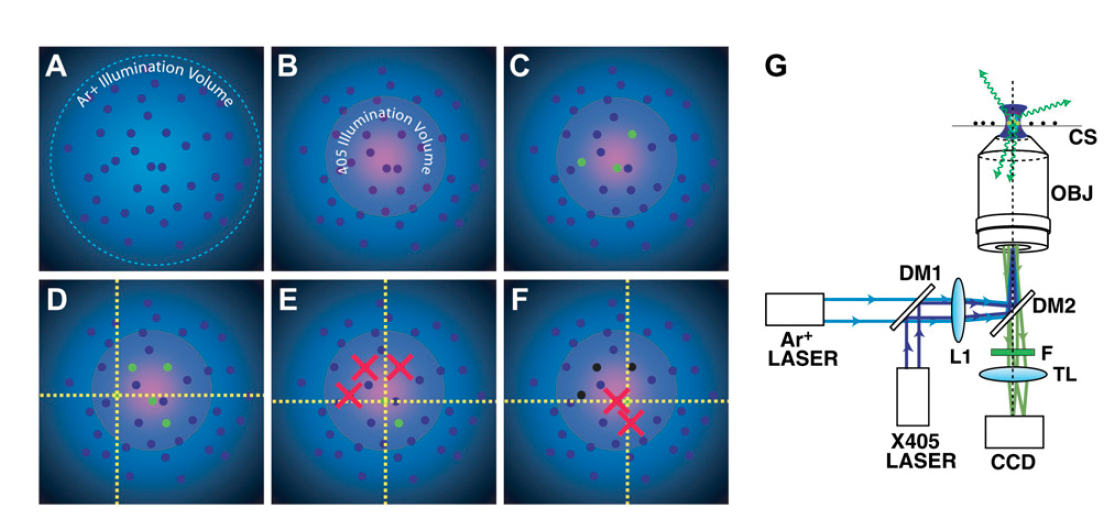
\includegraphics[width=\textwidth]{lm1}
\end{center}


A - пространственный профиль лазера, использующегося для считывания (в данном эксперименте аргоновый)

B - пространственный профиль лазера для активации (диодный лазер, 405 нм)
\end{frame}

\begin{frame}{Идея метода и отличие от других ДП методов}

Что общего в методах локализационной микроскопии и микроскопии сильно сфокусированных полей:
\begin{itemize}
\item  метод также основан на использовании фотопереключаемых флуоресцентных молекул;
\item также может применяться сканирование;
\item возможно совместно использование, например, с 4Pi-микроскопией.
\end{itemize}

Различия подходов:
\begin{itemize}
\item  стремимся к оптической изоляции молекул и работаем с сигналом от единичных молекул, снимается до нескольких тысяч картинок с одного места;
\item время перехода их темного в яркое состояние на несколько порядков больше  (от микросекунд в МСП до нескольких секунд в ЛМ), это обусловлено необходимостью оптической изоляции;
\item применяется метод статистической обработки информации по нахождению центров диска Эйри каждой отдельной молекулы.
\end{itemize}

\end{frame}

\begin{frame}{Схема эксперимента}

\begin{center}
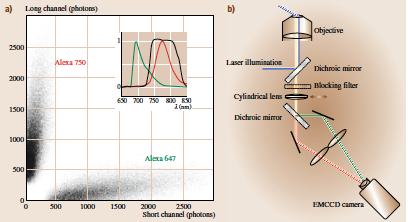
\includegraphics[width=0.9\textwidth]{lm21}
\end{center}

Излучение от двух единичных молекул регистрируются как вспышки.
\end{frame}

\begin{frame}{Последовательность событий}
\begin{center}
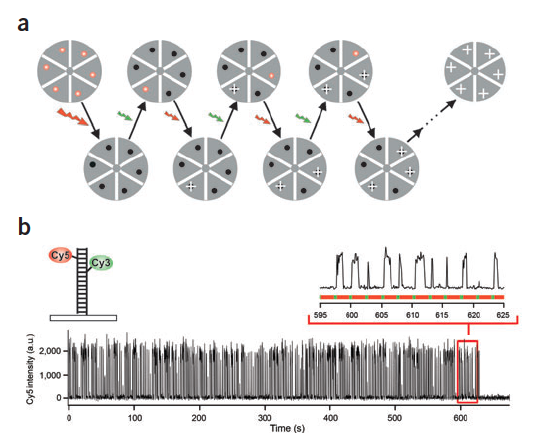
\includegraphics[width=0.9\textwidth]{lm14}
\end{center}
\end{frame}

\begin{frame}{Зависимость сигнала флуоресценции от времени}
\begin{center}
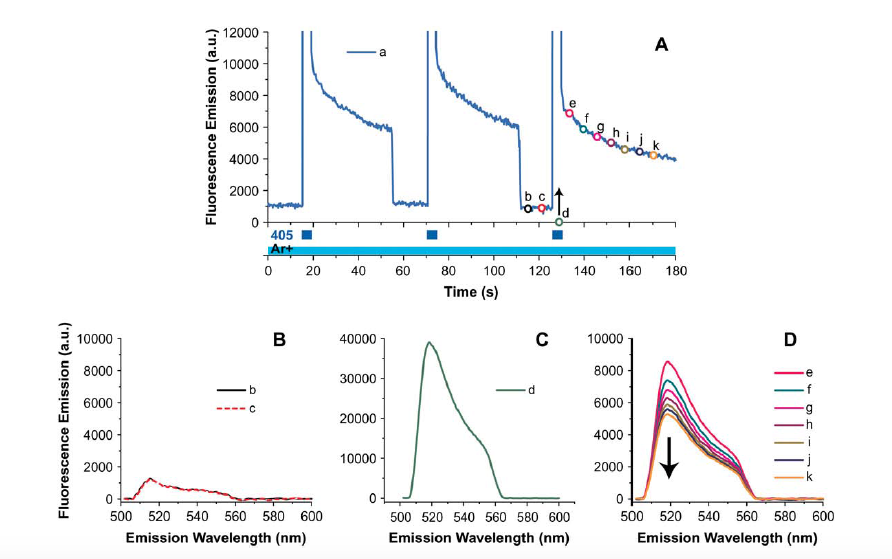
\includegraphics[width=0.9\textwidth]{lm2}

Длинный голубой прямоугольник показывает свечение аргонового лазера, короткие синие квадратики 405-нм диодный, использующийся для активации.

\end{center}
\end{frame}

\begin{frame}{Визуализация единичных молекул}
\begin{center}
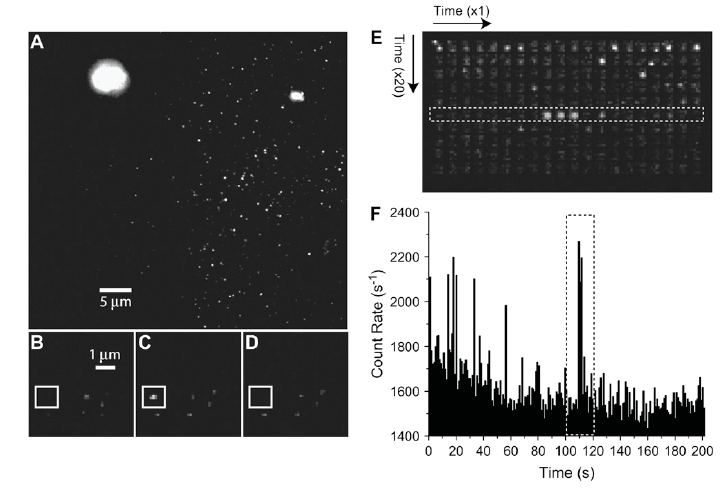
\includegraphics[width=0.9\textwidth]{lm5}

Делается около 200 (в данном эксперименте, в работах Cremer до нескольких тысяч) таких картинок, как А, затем они накладываются друг на друга

\end{center}
\end{frame}

\begin{frame}{Определение точки центра}
\begin{center}
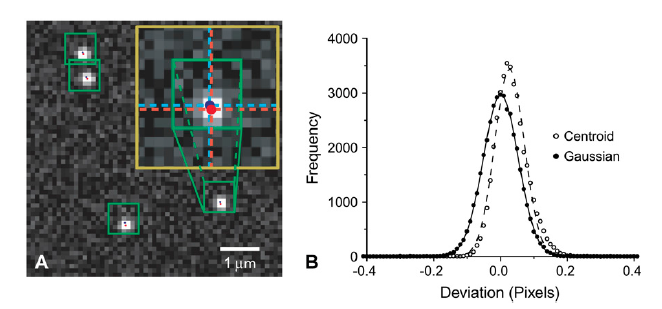
\includegraphics[width=0.9\textwidth]{lm3}

Точка центра определяется по подгоночной гауссовой кривой (в разных методах до 8-ми подгоночных параметров), с учетом шума, который имеет две причины: дробовой шум фотонов, сигналы флуоресценции от объектов за пределами исследуемой области.

\end{center}
\end{frame}

\begin{frame}{Результаты эксперимента}
\begin{columns}[c]
\column{6.5cm}
\begin{center}
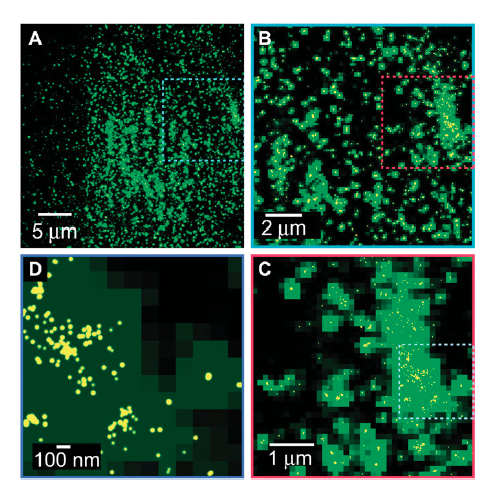
\includegraphics[width=0.9\textwidth]{lm9}
\end{center}
\column{6.5cm}
\begin{center}
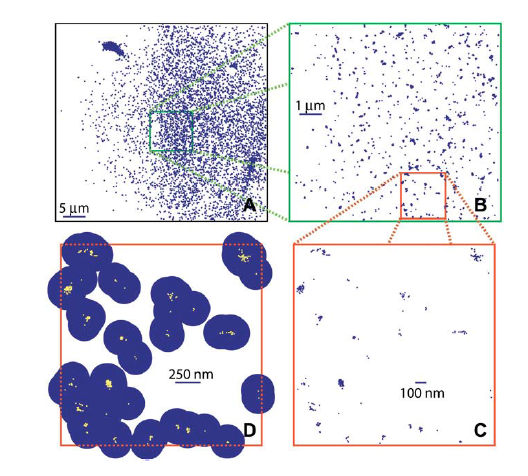
\includegraphics[width=0.9\textwidth]{lm10}
\end{center}
\end{columns}

Измерение координат расположения 48746 молекул PA-GFP, расположенных на стеклянной подложке. Ширина диска Эйри около 200 нм.
\end{frame}

\begin{frame}{Работы Zhuang}
\begin{center}
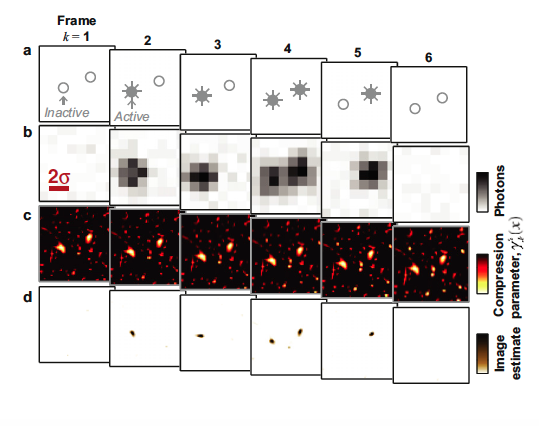
\includegraphics[width=0.8\textwidth]{lm8}

ФРТ микроскопа (второй ряд сверху) на порядок больше, чем получающийся в результате работы алгоритма STORM объект, соотносимый с положением молекулы.

\end{center}
\end{frame}

\begin{frame}{Работы Кремера}

Использование двухцветной схемы. В срезе толщиной 600 нм было насчитано 120000 белков ядра раковой клетки
\begin{center}
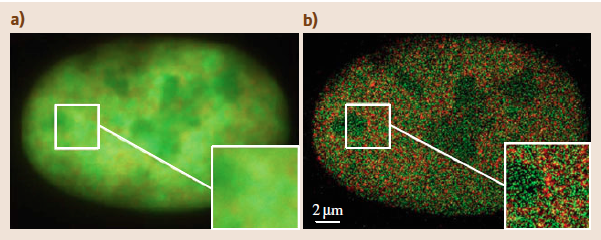
\includegraphics[width=0.7\textwidth]{ffm12}
\end{center}
Синапсин в гиппокампе
\begin{columns}[c]
\column{6.5cm}
\begin{center}
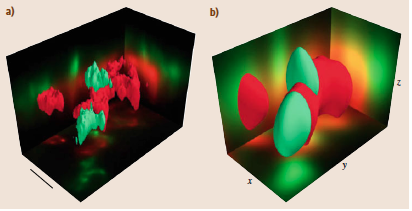
\includegraphics[width=0.5\textwidth]{ffm14}
\end{center}
\column{6.5cm}
{\tiny Гиппокамп (от др.-греч. ἱππόκαμπος — морской конёк) — часть лимбической системы головного мозга (обонятельного мозга). Участвует в механизмах формирования эмоций, консолидации памяти (то есть перехода кратковременной памяти в долговременную). Генерирует тета-ритм при удержании внимания.}
\end{columns}
\end{frame}

\begin{frame}{Сравнение методов и литература}
    
\begin{center}
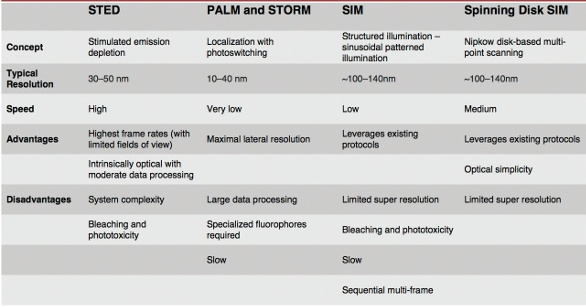
\includegraphics[width=0.5\textwidth]{comp}
\end{center}

 \begin{block}{Литература} \begin{itemize}
\item R. E. Thompson et al. Precise Nanometer Localization Analysis for Individual Fluorescent Probes. 2002. - Методика поиска центра диска Эйри и стат. обработки данных
\item S. T. Hess et al.Ultra-High Resolution Imaging by Fluorescence Photoactivation Localization Microscopy. 2006. Методика PALM
\item X. Zhuang Statistical Deconvolution for Superresolution Fluorescence Microscopy. 2012. Методика STORM
\item C. Cremer Optics Far Beyond diffraction Limit. 2012. Методика SPDM.
\end{itemize}
\end{block}
\end{frame}




\end{document}


\begin{frame}{}
\begin{columns}[c]
\column{6.5cm}
\begin{center}
\includegraphics[width=0.9\textwidth]{}
\end{center}
\column{6.5cm}
\begin{center}
\includegraphics[width=0.9\textwidth]{}
\end{center}
\end{columns}
\end{frame}

\begin{frame}{}
\begin{center}
\includegraphics[width=0.9\textwidth]{}
\end{center}
\end{frame}
